% Created by tikzDevice version 0.12.6 on 2025-03-31 20:33:58
% !TEX encoding = UTF-8 Unicode
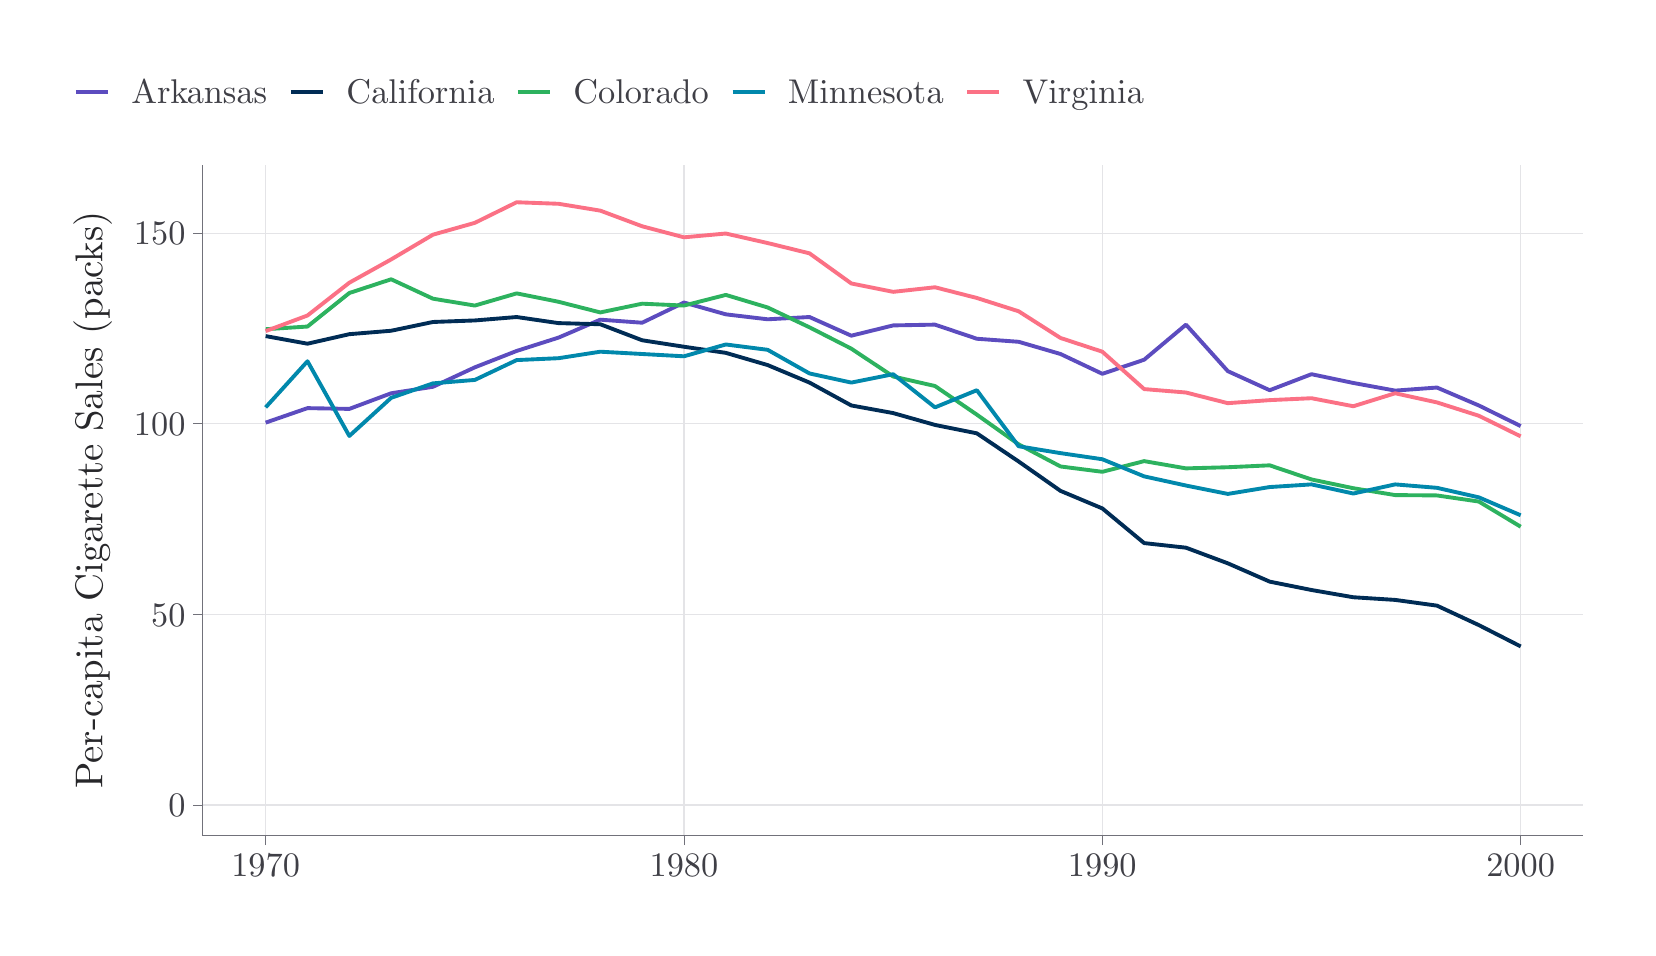
\begin{tikzpicture}[x=1pt,y=1pt]
\definecolor{fillColor}{RGB}{255,255,255}
\path[use as bounding box,fill=fillColor] (0,0) rectangle (578.16,325.21);
\begin{scope}
\path[clip] (  0.00,  0.00) rectangle (578.16,325.21);
\definecolor{drawColor}{RGB}{255,255,255}

\path[draw=drawColor,line width= 0.7pt,line join=round,line cap=round,fill=fillColor] (  0.00,  0.00) rectangle (578.16,325.21);
\end{scope}
\begin{scope}
\path[clip] ( 63.32, 33.29) rectangle (562.16,275.76);
\definecolor{drawColor}{RGB}{255,255,255}
\definecolor{fillColor}{RGB}{255,255,255}

\path[draw=drawColor,line width= 0.7pt,line join=round,line cap=round,fill=fillColor] ( 63.32, 33.29) rectangle (562.16,275.76);
\definecolor{drawColor}{RGB}{228,228,231}

\path[draw=drawColor,line width= 0.4pt,line join=round] ( 63.32, 44.31) --
	(562.16, 44.31);

\path[draw=drawColor,line width= 0.4pt,line join=round] ( 63.32,113.19) --
	(562.16,113.19);

\path[draw=drawColor,line width= 0.4pt,line join=round] ( 63.32,182.08) --
	(562.16,182.08);

\path[draw=drawColor,line width= 0.4pt,line join=round] ( 63.32,250.96) --
	(562.16,250.96);

\path[draw=drawColor,line width= 0.4pt,line join=round] ( 85.99, 33.29) --
	( 85.99,275.76);

\path[draw=drawColor,line width= 0.4pt,line join=round] (237.16, 33.29) --
	(237.16,275.76);

\path[draw=drawColor,line width= 0.4pt,line join=round] (388.32, 33.29) --
	(388.32,275.76);

\path[draw=drawColor,line width= 0.4pt,line join=round] (539.49, 33.29) --
	(539.49,275.76);
\definecolor{drawColor}{RGB}{92,76,191}

\path[draw=drawColor,line width= 1.4pt,line join=round] ( 85.99,182.49) --
	(101.11,187.73) --
	(116.23,187.45) --
	(131.34,193.10) --
	(146.46,195.44) --
	(161.58,202.47) --
	(176.69,208.39) --
	(191.81,213.21) --
	(206.92,219.69) --
	(222.04,218.59) --
	(237.16,225.89) --
	(252.27,221.62) --
	(267.39,219.83) --
	(282.51,220.65) --
	(297.62,213.90) --
	(312.74,217.62) --
	(327.86,217.90) --
	(342.97,212.80) --
	(358.09,211.70) --
	(373.21,207.29) --
	(388.32,200.13) --
	(403.44,205.22) --
	(418.55,217.90) --
	(433.67,201.09) --
	(448.79,194.20) --
	(463.90,199.99) --
	(479.02,196.82) --
	(494.14,194.06) --
	(509.25,195.17) --
	(524.37,188.69) --
	(539.49,181.25);
\definecolor{drawColor}{RGB}{0,44,85}

\path[draw=drawColor,line width= 1.4pt,line join=round] ( 85.99,213.76) --
	(101.11,211.01) --
	(116.23,214.45) --
	(131.34,215.69) --
	(146.46,218.86) --
	(161.58,219.41) --
	(176.69,220.65) --
	(191.81,218.45) --
	(206.92,218.04) --
	(222.04,212.25) --
	(237.16,209.91) --
	(252.27,207.70) --
	(267.39,203.29) --
	(282.51,196.96) --
	(297.62,188.69) --
	(312.74,185.94) --
	(327.86,181.66) --
	(342.97,178.63) --
	(358.09,168.44) --
	(373.21,157.83) --
	(388.32,151.49) --
	(403.44,138.96) --
	(418.55,137.30) --
	(433.67,131.65) --
	(448.79,125.04) --
	(463.90,122.01) --
	(479.02,119.39) --
	(494.14,118.43) --
	(509.25,116.36) --
	(524.37,109.33) --
	(539.49,101.62);
\definecolor{drawColor}{RGB}{45,178,95}

\path[draw=drawColor,line width= 1.4pt,line join=round] ( 85.99,216.24) --
	(101.11,217.21) --
	(116.23,229.33) --
	(131.34,234.29) --
	(146.46,227.27) --
	(161.58,224.79) --
	(176.69,229.19) --
	(191.81,226.16) --
	(206.92,222.31) --
	(222.04,225.47) --
	(237.16,224.79) --
	(252.27,228.64) --
	(267.39,224.10) --
	(282.51,216.93) --
	(297.62,209.22) --
	(312.74,199.16) --
	(327.86,195.72) --
	(342.97,185.38) --
	(358.09,174.64) --
	(373.21,166.65) --
	(388.32,164.72) --
	(403.44,168.58) --
	(418.55,165.96) --
	(433.67,166.37) --
	(448.79,167.06) --
	(463.90,161.96) --
	(479.02,158.79) --
	(494.14,156.31) --
	(509.25,156.18) --
	(524.37,153.97) --
	(539.49,144.88);
\definecolor{drawColor}{RGB}{1,136,172}

\path[draw=drawColor,line width= 1.4pt,line join=round] ( 85.99,188.00) --
	(101.11,204.67) --
	(116.23,177.67) --
	(131.34,191.45) --
	(146.46,196.68) --
	(161.58,197.92) --
	(176.69,205.09) --
	(191.81,205.77) --
	(206.92,208.12) --
	(222.04,207.29) --
	(237.16,206.46) --
	(252.27,210.73) --
	(267.39,208.80) --
	(282.51,200.26) --
	(297.62,196.96) --
	(312.74,199.99) --
	(327.86,188.00) --
	(342.97,194.20) --
	(358.09,173.95) --
	(373.21,171.47) --
	(388.32,169.26) --
	(403.44,163.07) --
	(418.55,159.76) --
	(433.67,156.73) --
	(448.79,159.21) --
	(463.90,160.17) --
	(479.02,156.87) --
	(494.14,160.17) --
	(509.25,158.93) --
	(524.37,155.49) --
	(539.49,149.01);
\definecolor{drawColor}{RGB}{251,113,133}

\path[draw=drawColor,line width= 1.4pt,line join=round] ( 85.99,215.56) --
	(101.11,221.20) --
	(116.23,233.05) --
	(131.34,241.46) --
	(146.46,250.41) --
	(161.58,254.68) --
	(176.69,262.12) --
	(191.81,261.57) --
	(206.92,259.09) --
	(222.04,253.44) --
	(237.16,249.45) --
	(252.27,250.82) --
	(267.39,247.38) --
	(282.51,243.66) --
	(297.62,232.78) --
	(312.74,229.75) --
	(327.86,231.40) --
	(342.97,227.54) --
	(358.09,222.72) --
	(373.21,213.08) --
	(388.32,208.12) --
	(403.44,194.61) --
	(418.55,193.37) --
	(433.67,189.52) --
	(448.79,190.62) --
	(463.90,191.31) --
	(479.02,188.41) --
	(494.14,193.10) --
	(509.25,189.79) --
	(524.37,184.97) --
	(539.49,177.53);
\end{scope}
\begin{scope}
\path[clip] (  0.00,  0.00) rectangle (578.16,325.21);
\definecolor{drawColor}{RGB}{113,113,122}

\path[draw=drawColor,line width= 0.3pt,line join=round] ( 63.32, 33.29) --
	( 63.32,275.76);
\end{scope}
\begin{scope}
\path[clip] (  0.00,  0.00) rectangle (578.16,325.21);
\definecolor{drawColor}{RGB}{63,63,70}

\node[text=drawColor,anchor=base east,inner sep=0pt, outer sep=0pt, scale=  1.24] at ( 57.02, 40.02) {0};

\node[text=drawColor,anchor=base east,inner sep=0pt, outer sep=0pt, scale=  1.24] at ( 57.02,108.91) {50};

\node[text=drawColor,anchor=base east,inner sep=0pt, outer sep=0pt, scale=  1.24] at ( 57.02,177.79) {100};

\node[text=drawColor,anchor=base east,inner sep=0pt, outer sep=0pt, scale=  1.24] at ( 57.02,246.68) {150};
\end{scope}
\begin{scope}
\path[clip] (  0.00,  0.00) rectangle (578.16,325.21);
\definecolor{drawColor}{RGB}{113,113,122}

\path[draw=drawColor,line width= 0.3pt,line join=round] ( 59.82, 44.31) --
	( 63.32, 44.31);

\path[draw=drawColor,line width= 0.3pt,line join=round] ( 59.82,113.19) --
	( 63.32,113.19);

\path[draw=drawColor,line width= 0.3pt,line join=round] ( 59.82,182.08) --
	( 63.32,182.08);

\path[draw=drawColor,line width= 0.3pt,line join=round] ( 59.82,250.96) --
	( 63.32,250.96);
\end{scope}
\begin{scope}
\path[clip] (  0.00,  0.00) rectangle (578.16,325.21);
\definecolor{drawColor}{RGB}{113,113,122}

\path[draw=drawColor,line width= 0.3pt,line join=round] ( 63.32, 33.29) --
	(562.16, 33.29);
\end{scope}
\begin{scope}
\path[clip] (  0.00,  0.00) rectangle (578.16,325.21);
\definecolor{drawColor}{RGB}{113,113,122}

\path[draw=drawColor,line width= 0.3pt,line join=round] ( 85.99, 29.79) --
	( 85.99, 33.29);

\path[draw=drawColor,line width= 0.3pt,line join=round] (237.16, 29.79) --
	(237.16, 33.29);

\path[draw=drawColor,line width= 0.3pt,line join=round] (388.32, 29.79) --
	(388.32, 33.29);

\path[draw=drawColor,line width= 0.3pt,line join=round] (539.49, 29.79) --
	(539.49, 33.29);
\end{scope}
\begin{scope}
\path[clip] (  0.00,  0.00) rectangle (578.16,325.21);
\definecolor{drawColor}{RGB}{63,63,70}

\node[text=drawColor,anchor=base,inner sep=0pt, outer sep=0pt, scale=  1.24] at ( 85.99, 18.42) {1970};

\node[text=drawColor,anchor=base,inner sep=0pt, outer sep=0pt, scale=  1.24] at (237.16, 18.42) {1980};

\node[text=drawColor,anchor=base,inner sep=0pt, outer sep=0pt, scale=  1.24] at (388.32, 18.42) {1990};

\node[text=drawColor,anchor=base,inner sep=0pt, outer sep=0pt, scale=  1.24] at (539.49, 18.42) {2000};
\end{scope}
\begin{scope}
\path[clip] (  0.00,  0.00) rectangle (578.16,325.21);
\definecolor{drawColor}{RGB}{39,39,42}

\node[text=drawColor,rotate= 90.00,anchor=base,inner sep=0pt, outer sep=0pt, scale=  1.40] at ( 27.00,154.52) {Per-capita Cigarette Sales (packs)};
\end{scope}
\begin{scope}
\path[clip] (  0.00,  0.00) rectangle (578.16,325.21);
\definecolor{drawColor}{RGB}{255,255,255}
\definecolor{fillColor}{RGB}{255,255,255}

\path[draw=drawColor,line width= 0.7pt,line join=round,line cap=round,fill=fillColor] ( 16.00,289.76) rectangle (403.46,309.22);
\end{scope}
\begin{scope}
\path[clip] (  0.00,  0.00) rectangle (578.16,325.21);
\definecolor{drawColor}{RGB}{255,255,255}
\definecolor{fillColor}{RGB}{255,255,255}

\path[draw=drawColor,line width= 0.7pt,line join=round,line cap=round,fill=fillColor] ( 16.00,294.76) rectangle ( 30.45,309.22);
\definecolor{drawColor}{RGB}{92,76,191}

\path[draw=drawColor,line width= 1.4pt,line join=round] ( 17.45,301.99) -- ( 29.01,301.99);
\end{scope}
\begin{scope}
\path[clip] (  0.00,  0.00) rectangle (578.16,325.21);
\definecolor{drawColor}{RGB}{255,255,255}
\definecolor{fillColor}{RGB}{255,255,255}

\path[draw=drawColor,line width= 0.7pt,line join=round,line cap=round,fill=fillColor] ( 93.68,294.76) rectangle (108.14,309.22);
\definecolor{drawColor}{RGB}{0,44,85}

\path[draw=drawColor,line width= 1.4pt,line join=round] ( 95.13,301.99) -- (106.69,301.99);
\end{scope}
\begin{scope}
\path[clip] (  0.00,  0.00) rectangle (578.16,325.21);
\definecolor{drawColor}{RGB}{255,255,255}
\definecolor{fillColor}{RGB}{255,255,255}

\path[draw=drawColor,line width= 0.7pt,line join=round,line cap=round,fill=fillColor] (175.72,294.76) rectangle (190.17,309.22);
\definecolor{drawColor}{RGB}{45,178,95}

\path[draw=drawColor,line width= 1.4pt,line join=round] (177.17,301.99) -- (188.73,301.99);
\end{scope}
\begin{scope}
\path[clip] (  0.00,  0.00) rectangle (578.16,325.21);
\definecolor{drawColor}{RGB}{255,255,255}
\definecolor{fillColor}{RGB}{255,255,255}

\path[draw=drawColor,line width= 0.7pt,line join=round,line cap=round,fill=fillColor] (253.27,294.76) rectangle (267.72,309.22);
\definecolor{drawColor}{RGB}{1,136,172}

\path[draw=drawColor,line width= 1.4pt,line join=round] (254.71,301.99) -- (266.27,301.99);
\end{scope}
\begin{scope}
\path[clip] (  0.00,  0.00) rectangle (578.16,325.21);
\definecolor{drawColor}{RGB}{255,255,255}
\definecolor{fillColor}{RGB}{255,255,255}

\path[draw=drawColor,line width= 0.7pt,line join=round,line cap=round,fill=fillColor] (338.10,294.76) rectangle (352.56,309.22);
\definecolor{drawColor}{RGB}{251,113,133}

\path[draw=drawColor,line width= 1.4pt,line join=round] (339.55,301.99) -- (351.11,301.99);
\end{scope}
\begin{scope}
\path[clip] (  0.00,  0.00) rectangle (578.16,325.21);
\definecolor{drawColor}{RGB}{63,63,70}

\node[text=drawColor,anchor=base west,inner sep=0pt, outer sep=0pt, scale=  1.24] at ( 37.45,297.70) {Arkansas};
\end{scope}
\begin{scope}
\path[clip] (  0.00,  0.00) rectangle (578.16,325.21);
\definecolor{drawColor}{RGB}{63,63,70}

\node[text=drawColor,anchor=base west,inner sep=0pt, outer sep=0pt, scale=  1.24] at (115.14,297.70) {California};
\end{scope}
\begin{scope}
\path[clip] (  0.00,  0.00) rectangle (578.16,325.21);
\definecolor{drawColor}{RGB}{63,63,70}

\node[text=drawColor,anchor=base west,inner sep=0pt, outer sep=0pt, scale=  1.24] at (197.17,297.70) {Colorado};
\end{scope}
\begin{scope}
\path[clip] (  0.00,  0.00) rectangle (578.16,325.21);
\definecolor{drawColor}{RGB}{63,63,70}

\node[text=drawColor,anchor=base west,inner sep=0pt, outer sep=0pt, scale=  1.24] at (274.72,297.70) {Minnesota};
\end{scope}
\begin{scope}
\path[clip] (  0.00,  0.00) rectangle (578.16,325.21);
\definecolor{drawColor}{RGB}{63,63,70}

\node[text=drawColor,anchor=base west,inner sep=0pt, outer sep=0pt, scale=  1.24] at (359.56,297.70) {Virginia};
\end{scope}
\end{tikzpicture}
